% Source : http://tex.stackexchange.com/questions/30032/highlighting-diagonal-of-a-square-matrix

\documentclass{article}
	\usepackage{tikz}
	\usetikzlibrary{matrix}
	%\usetikzlibrary{shapes} %Uncomment if you want additional shapes


\begin{document}

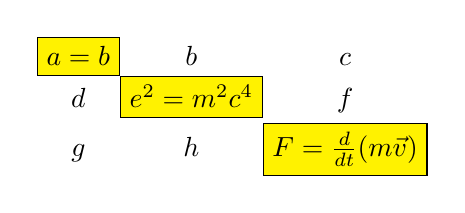
\begin{tikzpicture}
\matrix (m) [matrix of math nodes]{
	| [draw,fill= yellow] | a=b & b                               & c\\
	d                           &|[draw,fill= yellow]| e^2=m^2c^4 & f\\
	g                           & h                               &|[draw,fill= yellow]|F = \frac{d}{dt}{(m\vec{v})}\\
};
\end{tikzpicture}

\end{document}
